\section{Populating Tables With Data}

Now that we have successfully created all the necessary data, it is time to fill them with data. We will use a variety of different methods to import data to our tables.

\subsection{Populating Users}

We retrieved a large excel file containing over three hundred thousand users' data from the internet, and using the PL/SQL Developer tool called ODBC importer we imported the data which we needed into the users table. Not all of the columns provided were necessary to us, so figure \ref{users-odbc} shows which columns we used. The excel file which we used can be found in \verb`/data/users/user_list.xlsx`.

\begin{figure}[hbtp]
	\centering
	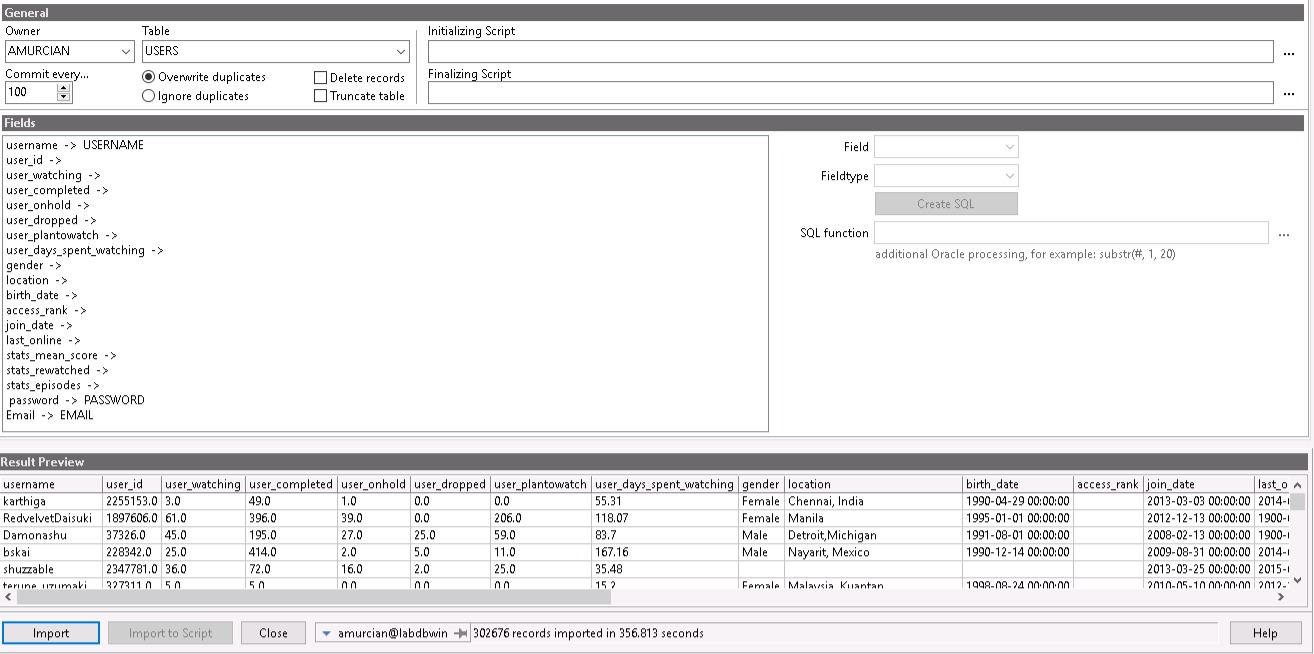
\includegraphics[width=\linewidth]{images/users_odbc.jpeg}
	\caption{A screenshot showing how the ODBC importer imported our data}
	\label{users-odbc}
\end{figure}

\subsection{Populating Topics}

We were able to find a large list with 1,547 topics which Quora uses to organise their questions. We obtained it in the form of a plain text file with one line for each topic name. Since it contains duplicates, we can must first remove these. Then we generate some randomised description using the python module called \verb`lorem`. This python code shows exactly how the insert statements were generated. The generated SQL code can be found at \verb`/sql/insert/topics.sql`

\VerbatimInput[label=\fbox{\color{Black}/data/topics/topics\_to\_insert.py}]{../../data/topics/topics_to_insert.py}